%%%%%%%%%%%%%%%%%%%%%%%%%%%%%%%%%%%%%%%%%%%%%%%%%%%%%%%%%%%%%%%%%%%%%%%
%
%   Presentation of Beamer UNL Theme
%   Beamer Presentation by Chris Bourke
%
%%%%%%%%%%%%%%%%%%%%%%%%%%%%%%%%%%%%%%%%%%%%%%%%%%%%%%%%%%%%%%%%%%%%%%%

\documentclass{beamer}

\usetheme[hideothersubsections]{UNLTheme}
\usepackage[postscript]{ucs}
\usepackage[utf8x]{inputenc}

\title{Performance Modeling and
Design of Computer Systems- Ch 4 \\
Generating Random Variables
for Simulation
}
\author{Debobroto Das Robin} %
\institute{Kent State University}
\date{Spring 2020}




\begin{document}

%{% open a Local TeX Group
%\setbeamertemplate{sidebar}{}
\begin{frame}
        \titlepage
        \begin{center}
    \href{mailto:drobin@kent.edu}{\color{blue}{\texttt{drobin@kent.edu}}}
        \end{center}
\end{frame}

\begin{frame}
\frametitle{Overview} % Table of contents slide, comment this block out to remove it
\tableofcontents % Throughout your presentation, if you choose to use \section{} and \subsection{} commands, these will automatically be printed on this slide as an overview of your presentation
\end{frame}



\section{Introduction}



\begin{frame}
    \frametitle{Random Variable Generation}
    \framesubtitle{\textbf{\textit{}}}
	\begin{itemize}
	
		\item \textbf{Problem} : Assume a system in which  
			\begin{itemize}
			\item \textbf{interarrival times of jobs }are well modeled by an
						\textbf{Exponential distribution } 
			\item \textbf{Job sizes} (service requirements) are well modeled
					by a \textbf{Normal distribution}.
			\item We want to simulate the system 
			\end{itemize}
		\item We need to be able to generate instances of 
			\begin{itemize}
			\item \textbf{Exponential distribution }  \&
			\item \textbf{Job sizes} (service requirements) are well modeled
				\textbf{Normal distribution}.
			\end{itemize}
		\item \textbf{Solution } : 2 Basic maethods for generating random 						variables
			\begin{itemize}
			\item Assuming we already have a generator of 										\textbf{\textit{Uniform(0,1)}} ($u \: \epsilon \: U(0,1)$) 
			random variables 
			\end{itemize}
		\item 2 methods are
			\begin{itemize}
				\item Inverse-Transform Method
				\item Accept-Reject Method

			\end{itemize}
		  
	\end{itemize}	    
    
\end{frame}

\section{Inverse-Transform Method}



\begin{frame}
    \frametitle{Inverse-Transform Method}
    \framesubtitle{Basics}
    \textbf{Idea}: Map each element $u$ generated by uniform distribution to some x of desired distribution
	\begin{itemize}
		\item This method assumes that we know the
		\begin{itemize}
		\item c.d.f. (cumulative distribution function), $F_X (x) = P( X \leq 				x)$, of the random variable $X$ that we are trying to generate, and
		\item that this distribution is easily invertible, namely that we can 				get $x$ from $F_X (x)$
		\end{itemize}
		\item 2 variations
		\begin{itemize}
		\item Continuous
		\item Discrete
		\end{itemize}
		
		  
	\end{itemize}	

\end{frame}

\subsection{Continuous Case}


\begin{frame}
    \frametitle{Inverse-Transform Method}
    \framesubtitle{Continuous Case}
	\begin{itemize}
		\item [Idea]: map each $u \: \epsilon \: U(0,1)$ generated to some $x$, 				where c.d.f is of $X$ is $F_x$.
		\item We already have uniform \textbf{random variable} generator system  
		\item $u \: \epsilon \: U(0,1) \rightarrow x \: \epsilon \: X(0,\inf) $
		\item we need to find the inverse transform that maps $u$ to $x$
		\item we want 
		\begin{equation}
		u =P\{0<U<u\} = P\{0<X<x\} = F_x(x) 
		\end{equation}
		\begin{equation}
		u = F_x(x) \Longrightarrow x = {{F}_{x}}^{-1}(u)
		\end{equation}
		\item Algorithm \textbf{Inverse-Transform Method to generate r.v. X}
		\begin{itemize}
		\item Generate  $u \: \epsilon \: U(0,1)$
		\item $X = {{F}_{x}}^{-1}(u)$
		\end{itemize}
		  
	\end{itemize}	

\end{frame}


\begin{frame}
    \frametitle{Inverse-Transform Method}
    \framesubtitle{Continuous Case: Example exponential  distribution}
	\begin{itemize}
		\item Assume we want to get random variable $x$ that follows 						exponential distribution
		\item $F (x) = u$ \\
		$\Rightarrow 1- e^{-\lambda x} = u$ \\
		$\Rightarrow -\lambda x = ln (1-u)$ \\
		$\Rightarrow x = - \dfrac{1}{\lambda}  ln (1-u)$
	\item Given $u \: \epsilon \: U(0,1)$ , get $x$ from the formula
	\item $x $ is an instance of $X \sim Exp (\lambda)$
		  
	\end{itemize}	

\end{frame}

\subsection{Discrete Case}

\begin{frame}
    \frametitle{Inverse-Transform Method}
    \framesubtitle{Discrete Case}
	\begin{itemize}
		\item Same basic idea as continuous case
		\item We want $X$ such that
		{
		\begin{figure}
        \begin{center}
		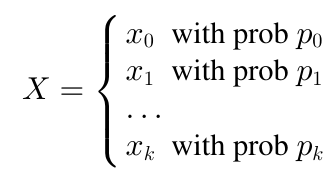
\includegraphics[scale=0.2]{images/discre_inv_teans_1.jpeg}
        \end{center}
		\end{figure}
		} 
		    
		{
		\begin{figure}
        \begin{center}
		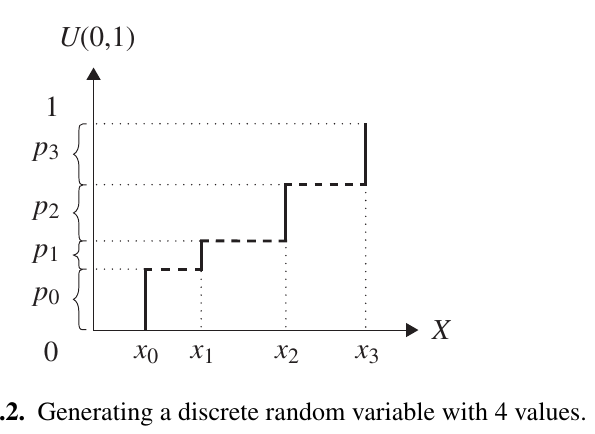
\includegraphics[scale=0.2]{images/discre_inv_teans_2.jpeg}
        \end{center}
		\end{figure}
		} 
		\item Solution 
		{
		\begin{figure}
        \begin{center}
		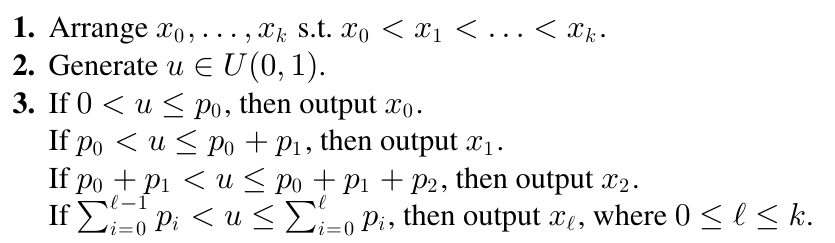
\includegraphics[scale=0.2]{images/discrete_rv_algo.jpg}
        \end{center}
		\end{figure}
		}
		  
	\end{itemize}	   
    
\end{frame}

\begin{frame}
    \frametitle{Inverse-Transform Method}
    \framesubtitle{Practical Consideration for Solution }
	\begin{itemize}
		\item Issues in the algorithm described in prev. page
		\begin{itemize}
		\item the eqn. is not closed form
		\item If X can take too many values $\rightarrow$ too many iterations
		\end{itemize}
		\item Solution: Find an inverse transform like continuous case
		
		  
	\end{itemize}	   
    
\end{frame}


\section{Accept-Reject Method}

\begin{frame}
    \frametitle{Accept-Reject Method}
    \framesubtitle{Basics }
	\begin{itemize}
		\item Applicable when, 
		\begin{itemize}
		\item we do not know the c.d.f., $F_X{x}$, but only know the p.d.f., 					$f_X ()$
		\item Ex: we want to generate a random variable from Normal 						distribution whose c.d.f. is unknown 

		\end{itemize}
		\item Idea: generate instances of the desired random variable, but throwing away (rejecting) some of the generated instances until the desired p.d.f (or p.m.f.) is met. 
		\item Two cases
		\begin{itemize}
		\item Discrete
		\item Continuous
		\end{itemize}
		  
	\end{itemize}	   
    
\end{frame}

\subsection{Discrete Case}


\begin{frame}
    \frametitle{Accept-Reject Method}
    \framesubtitle{Discrete Case }
	\begin{itemize}
		\item Given: Efficient method for generating random variable Q with probability mass function {$q_j , j:$discrete}, where $q_j = P {Q = j}$
\item Output: Random variable $P$ with probability mass function {$p_j , j:$discrete}, where $p_j = P {P = j}$
\item Requirement: For all j , we must have $q_j > 0 \Longleftarrow\Longrightarrow p_j > 0$. That is, P and Q take on
the same set of values
\item Example
		{
		\begin{figure}
        \begin{center}
		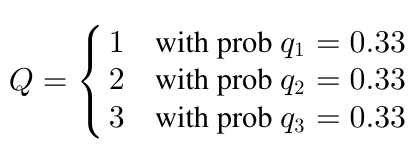
\includegraphics[scale=0.2]{images/accept_reject_discrete_q.jpg}
        \end{center}
		\end{figure}
		} 
		{
		\begin{figure}
        \begin{center}
		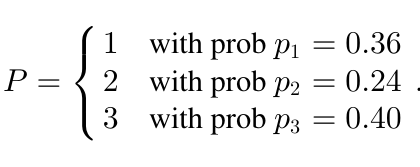
\includegraphics[scale=0.2]{images/accept_reject_discrete_p.jpg}
        \end{center}
		\end{figure}
		} 
		  
	\end{itemize}	   
    
\end{frame}


\begin{frame}
    \frametitle{Accept-Reject Method}
    \framesubtitle{Discrete Case: algorithm  }
	\begin{itemize}
		\item Algorithm
		{
		\begin{figure}
        \begin{center}
		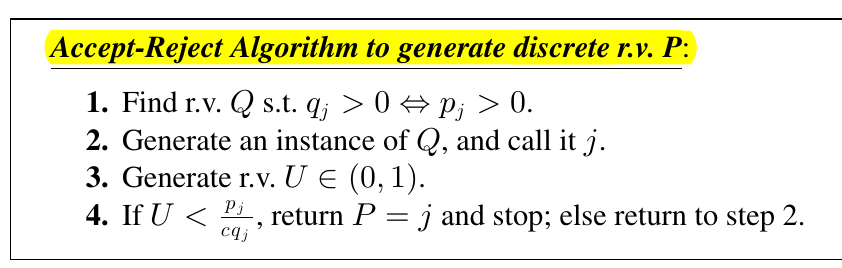
\includegraphics[scale=0.2]{images/accept_reject_algo.jpg}
        \end{center}
		\end{figure}
		} 
		Here c  $ > $1 
		\item Proof details in book page 74
		  
	\end{itemize}	   
    
\end{frame}
\subsection{Continuous Case}


\begin{frame}
    \frametitle{Accept-Reject Method}
    \framesubtitle{Continuous Case  }
	\begin{itemize}
	\item Given: We know how to generate $Y$ with probability density function $f_Y (t)$.
\item Goal: To generate $X$ with p.d.f. $f_X (t)$.
\item Requirement: For all $t$, $f_Y (t) > 0 \Longleftarrow\Longrightarrow f_X (t) > 0$

		\item Algorithm
		{
		\begin{figure}
        \begin{center}
		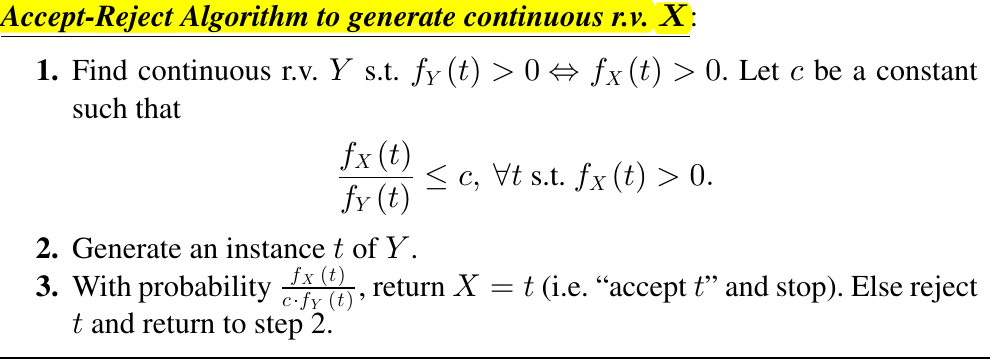
\includegraphics[scale=0.3]{images/accept_reject_cont_case_algo.jpg}
        \end{center}
		\end{figure}
		} 		  
	\end{itemize}	   
    
\end{frame}
    
\end{document}